
\section{Trắc địa}
\begin{defn}
    Một đường tham số tốc độ đơn vị $\gamma: I\to \hh$ được gọi là một \textbf{trắc địa} nếu với mọi $t,s \in I$ với $t\leq s$, ta có
    \[\rho(\gamma(s),\gamma(t)) = h(\gamma|_{[t,s]}).\]
\end{defn}
\begin{remark*}
    Đường tham số $\gamma: I\to \hh$ được gọi là có tốc độ đơn vị
    nếu với mọi $t\in I$ thì \[1 = |\gamma'(t)|_{hyp} = \dfrac{|\gamma'(t)|}{\im(\gamma(t))} \Leftrightarrow |\gamma'(t)| = \im(\gamma(t)).\]
\end{remark*}
Trong định nghĩa trên, nhận xét rằng $\gamma|_{[t,s]}$ là đường cong từ $\gamma(t)$ đến $\gamma(s)$. Do đó ta luôn có 
\[\rho(\gamma(t),\gamma(s)) \leq h(\gamma|_{[t,s]}).\]
Mặt khác, vì ta giả sử $\gamma$ là một đường tham số tốc độ đơn vị nên $h(\gamma_{[t,s]}) = s-t$.

Ta thấy rằng các đường trắc địa trong mặt phẳng hyperbolic $\hh$ là sự tương tự của các đoạn thẳng trong mặt phẳng Euclid $\R^2$.

Ta thường đồng nhất trắc địa $\gamma$ trong $\hh$ với vết của nó, và do đó, ta cũng gọi vết của trắc địa $\gamma$ là một trắc địa trong $\hh$.

\begin{exam*}
    Đường tham số $\gamma:\R \to \hh$ cho bởi $\gamma(t) = ie^{t}$ là một trắc địa của $\hh$. Vết của $\gamma$ là $\{ir~|~r\in \R_{>0}\}$.

    Thật vậy, ta có với mọi $t\in \R$ thì $|\gamma'(t)|_{hyp} = \dfrac{|\gamma'(t)|}{\im(\gamma(t))} = \dfrac{|ie^t|}{\im(ie^t)} = \dfrac{e^t}{e^t} = 1$.
    
    Chứng tỏ $\gamma$ là một đường tham số tốc độ đơn vị. 
    Nên với mọi $t\leq s$ thì \[h(\gamma|_{[t,s]}) = \int_t^s|\gamma'(t)|_{hyp}dt = s-t.\]

    Mặt khác, theo mệnh đề \ref{prop 2.1.8} thì $ \rho(\gamma(t),\gamma(s)) = \gamma(ie^t,ie^s) = \left|\ln{\dfrac{e^t}{e^s}}\right| = s-t$.

    Vì vậy $\rho(\gamma(t),\gamma(s)) = h(\gamma|_{[t,s]})$.
\end{exam*}
Ta muốn xác định tất cả các trắc địa của mặt phẳng hyperbolic $\hh$.
\begin{prop}\label{prop 2.2.3}
    Cho $T$ là một phép đẳng cự của $\hh$ và $\gamma$ là một trắc địa của $\hh$. Khi đó, đường tham số $T(\gamma)$ cũng là một trắc địa của $\hh$.
\end{prop}
\begin{proof}
    Giả sử $\gamma: I \to \hh$ là một trắc địa của $\hh$. Khi đó với mọi $t,s \in I, t \leq s$ thì
    \[\rho(\gamma(s),\gamma(t)) = h(\gamma_{[t,s]})\]
    
    Với $T$ là một đẳng cự trong $\hh$ thì $T\circ \gamma: I \to \hh, t \mapsto T(\gamma(t))$. Khi đó, với mọi $t,s \in I, t \leq s$, sử dụng mệnh đề \ref{prop 2.1.10} ta có
    \[\rho(T(\gamma(s)),T(\gamma(t))) = \rho(\gamma(s),\gamma(t)) = h(\gamma_{[t,s]}) = h(T(\gamma)|_{[t,s]})\]
    Chứng tỏ $T(\gamma)$ cũng là một trắc địa của $\hh$.
\end{proof}
\begin{cor}\label{cor 2.2.4}
    Với mỗi ma trận $\matt \in \SL(2,\R)$, đường cong 
    \[\left\{\dfrac{iar+b}{icr+d}: r \in \R_{>0}\right\} \subset \hh\]
    là một trắc địa của $\hh$.
\end{cor}
\begin{proof}
    Ta có $T(z) = \dfrac{az+b}{cz+d}$ là một đẳng cự trên $\hh$ và $\gamma: \R_{>0} \to \hh, t\mapsto ie^t$ là một trắc địa của $\hh$. Do đó theo mệnh đề \ref{prop 2.2.3} thì $T(\gamma)$ cũng là một trắc địa của $\hh$. Vết của $T(\gamma)$ là $\left\{\dfrac{iae^t+b}{ice^t+d}: t \in \R_{>0}\right\} = \left\{\dfrac{iar+b}{icr+d}: r \in \R_{>0}\right\}$.
\end{proof}
Ta muốn mô tả hình học cho các trắc địa của $\hh$ trong hệ quả trên. Muốn vậy, ta cần sử dụng một số kết quả cơ bản của phép biến đổi phân tuyến tính của $P^1(\C)$.
\begin{defn}
    Một \textbf{đường tròn suy rộng} trong $P^1(\C)$ là một đường tròn trong $\C$ hoặc hợp của một đường thẳng trong $\C$ với $\{\infty\}$.
\end{defn}
\begin{exam*}
    Một đường tròn suy rộng trong $P^1(\C)$ là $P^1(\R) = \R \cup \{\infty\}$.
\end{exam*}
Mệnh đề sau cho ta cách mô tả chung cho tất cả các đường tròn suy rộng.
\begin{prop}\label{prop 2.2.7}
    Đường tròn suy rộng trong $P^1(\C)$ là tập các điểm $[z:w]$ thoả mãn một phương trình có dạng
    \[(z\quad w)H\binom{\overline{z}}{\overline{w}} = 0\]
    trong đó $H \in \Mat(2,\C)$ là một ma trận Hermite, tức là $\overline{H} = H^T$.
\end{prop}
\begin{proof}
    Giả sử $C$ là một đường tròn suy rộng trong $\C$. Khi đó ta có hai trường hợp sau
    \begin{enumerate}
        \item $C$ là một đường tròn trong $\C$, giả sử tâm $\alpha \in \C$, bán kính $r>0$.

        Khi đó 
        $r^2 = |z-\alpha|^2 ~\forall z \in C$, tức là
        $r^2 = (z-\alpha)\overline{(z-\alpha)} = z\overline{z}-z\overline{\alpha} - \alpha \overline{z} + |\alpha|^2$.

        Do đó
        \[(z\quad 1)\begin{pmatrix}
            1 & -\overline{\alpha}\\
            -\alpha & |\alpha|^2-r^2
        \end{pmatrix}
        \begin{pmatrix}
            \overline{z}\\ 1
        \end{pmatrix} = 0\]
        với $\begin{pmatrix}
            1 & -\overline{\alpha}\\
            -\alpha & |\alpha|^2-r^2
        \end{pmatrix}$ là một ma trận Hermite.
        
        Vậy mọi $[z:w] \in C$ đều thoả mãn \[(z\quad w)\begin{pmatrix}
            1 & -\overline{\alpha}\\
            -\alpha & |\alpha|^2-r^2
        \end{pmatrix}\binom{\overline{z}}{\overline{w}} = 0.\]
        \item $C$ là hợp của một đường thẳng $L$ trong $\C$ với $\{\infty\}$, trong đó $L$ tạo với đường thẳng $\{z\in \C~|~\re(z) = r\}$ một góc $\theta$. Tức là $L = e^{i\theta}\{z\in \C~|~\re(z) = r\}.$

        Khi đó $z\in L \Leftrightarrow \re(e^{-i\theta}z) = r \Leftrightarrow e^{i\theta}\overline{z} + e^{-i\theta}z - 2r = 0 \Leftrightarrow (z \quad 1)\begin{pmatrix}
            0 & e^{-i\theta}\\
            e^{i\theta} & -2r
        \end{pmatrix}\begin{pmatrix}
            \overline{z} \\ 1
        \end{pmatrix} = 0$,
        
        trong đó $\begin{pmatrix}
            0 & e^{-i\theta}\\
            e^{i\theta} & -2r
        \end{pmatrix}$ là một ma trận Hermite.

        Nói riêng, $(1 \quad 0)\begin{pmatrix}
            0 & e^{-i\theta}\\
            e^{i\theta} & -2r
        \end{pmatrix}\begin{pmatrix}
            1 \\ 0
        \end{pmatrix} = 0.$

        Do đó, mọi điểm $[z:w]$ của $C = L \cup \{\infty\}$ đều thoả mãn 
        $(z\quad w)\begin{pmatrix}
            0 & e^{-i\theta}\\
            e^{i\theta} & -2r
        \end{pmatrix}\begin{pmatrix}
            \overline{z}\\ \overline{w}
        \end{pmatrix} = 0$. 
    \end{enumerate}
\end{proof}
Như vậy, các ma trận Hermite tương ứng với các đường tròn suy rộng $C$ trong $P^1(\C)$ có dạng 
\begin{enumerate}
    \item $H = \begin{pmatrix}
            1 & -\overline{\alpha}\\
            -\alpha & |\alpha|^2-r^2
        \end{pmatrix}$ nếu $C$ là đường tròn tâm $\alpha$ bán kính $r$.
    \item $H = \begin{pmatrix}
            0 & e^{-i\theta}\\
            e^{i\theta} & -2r
        \end{pmatrix}$ với $C$ là hợp của một đường thẳng trong $\C$ với $\{\infty\}$.
\end{enumerate}
Khái niệm ma trận Hermite là phiên bản phức của khái niệm ma trận đối xứng hệ số thực. Hơn nữa, một ma trận $\hh \in \Mat(2,\R)$ là một ma trận Hermite khi và chỉ khi nó là một ma trận đối xứng. 
\begin{prop}\label{prop 2.2.8}
    Cho $A \in \GL(2,\C)$. Khi đó, phép biến đổi xạ ảnh $T_A: P^1(\C)\to P^1(\C)$ biến một đường tròn suy rộng thành một đường tròn suy rộng.
\end{prop}
\begin{proof}
    Giả sử $C$ là một đường tròn suy rộng trong $P^1(\C)$. Khi đó, mọi điểm xạ ảnh $[z:w] \in C$ đều thoả mãn \[(z\quad w)H\binom{\overline{z}}{\overline{w}} = 0,\]
    trong đó $H$ là một ma trận Hermite.
    
    Đặt $[z':w'] = T_A([z:w])$, khi đó $\begin{pmatrix}
        z'\\w'
    \end{pmatrix} = A\begin{pmatrix}
        z\\w
    \end{pmatrix} \Leftrightarrow \begin{pmatrix}
        z\\w
    \end{pmatrix} = B\begin{pmatrix}
        z'\\w'
    \end{pmatrix}$, với $B = A^{-1}$.

    Khi đó
    \begin{align*}
        (z\quad w)H\begin{pmatrix}
            \overline{z}\\
            \overline{w}
        \end{pmatrix} = 0 \Leftrightarrow (z' \quad w')B^TH\overline{B}\begin{pmatrix}
            \overline{z'}\\
            \overline{w'}
        \end{pmatrix} = 0.
    \end{align*}
    Vì $(B^TH\overline{B})^T = \overline{B}^TH^TB = \overline{B^T}~\overline{H}~ \overline{\overline{B}}=\overline{B^TH\overline{B}}$, nên nó là một ma trận Hermite. 
    
    Do đó $T_A(C)$ là một đường tròn suy rộng trong $P^1(\C)$.
\end{proof}
\begin{cor}\label{cor 2.2.9}
    Với mỗi ma trận $\matt \in \SL(2,\R)$, trắc địa 
    \[\left\{\dfrac{iar+b}{icr+d}: r \in \R_{>0}\right\} \subset \hh\]
    chứa trong một đường thẳng hoặc một đường tròn của $\C$.
\end{cor}
Để xác định các trắc địa của mặt phẳng hyperbolic $\hh$, các đường tròn suy rộng mà chúng ta quan tâm đặc biệt là các đường tròn suy rộng vuông góc với $P^1(\R)$. 
\begin{figure}
    \centering
    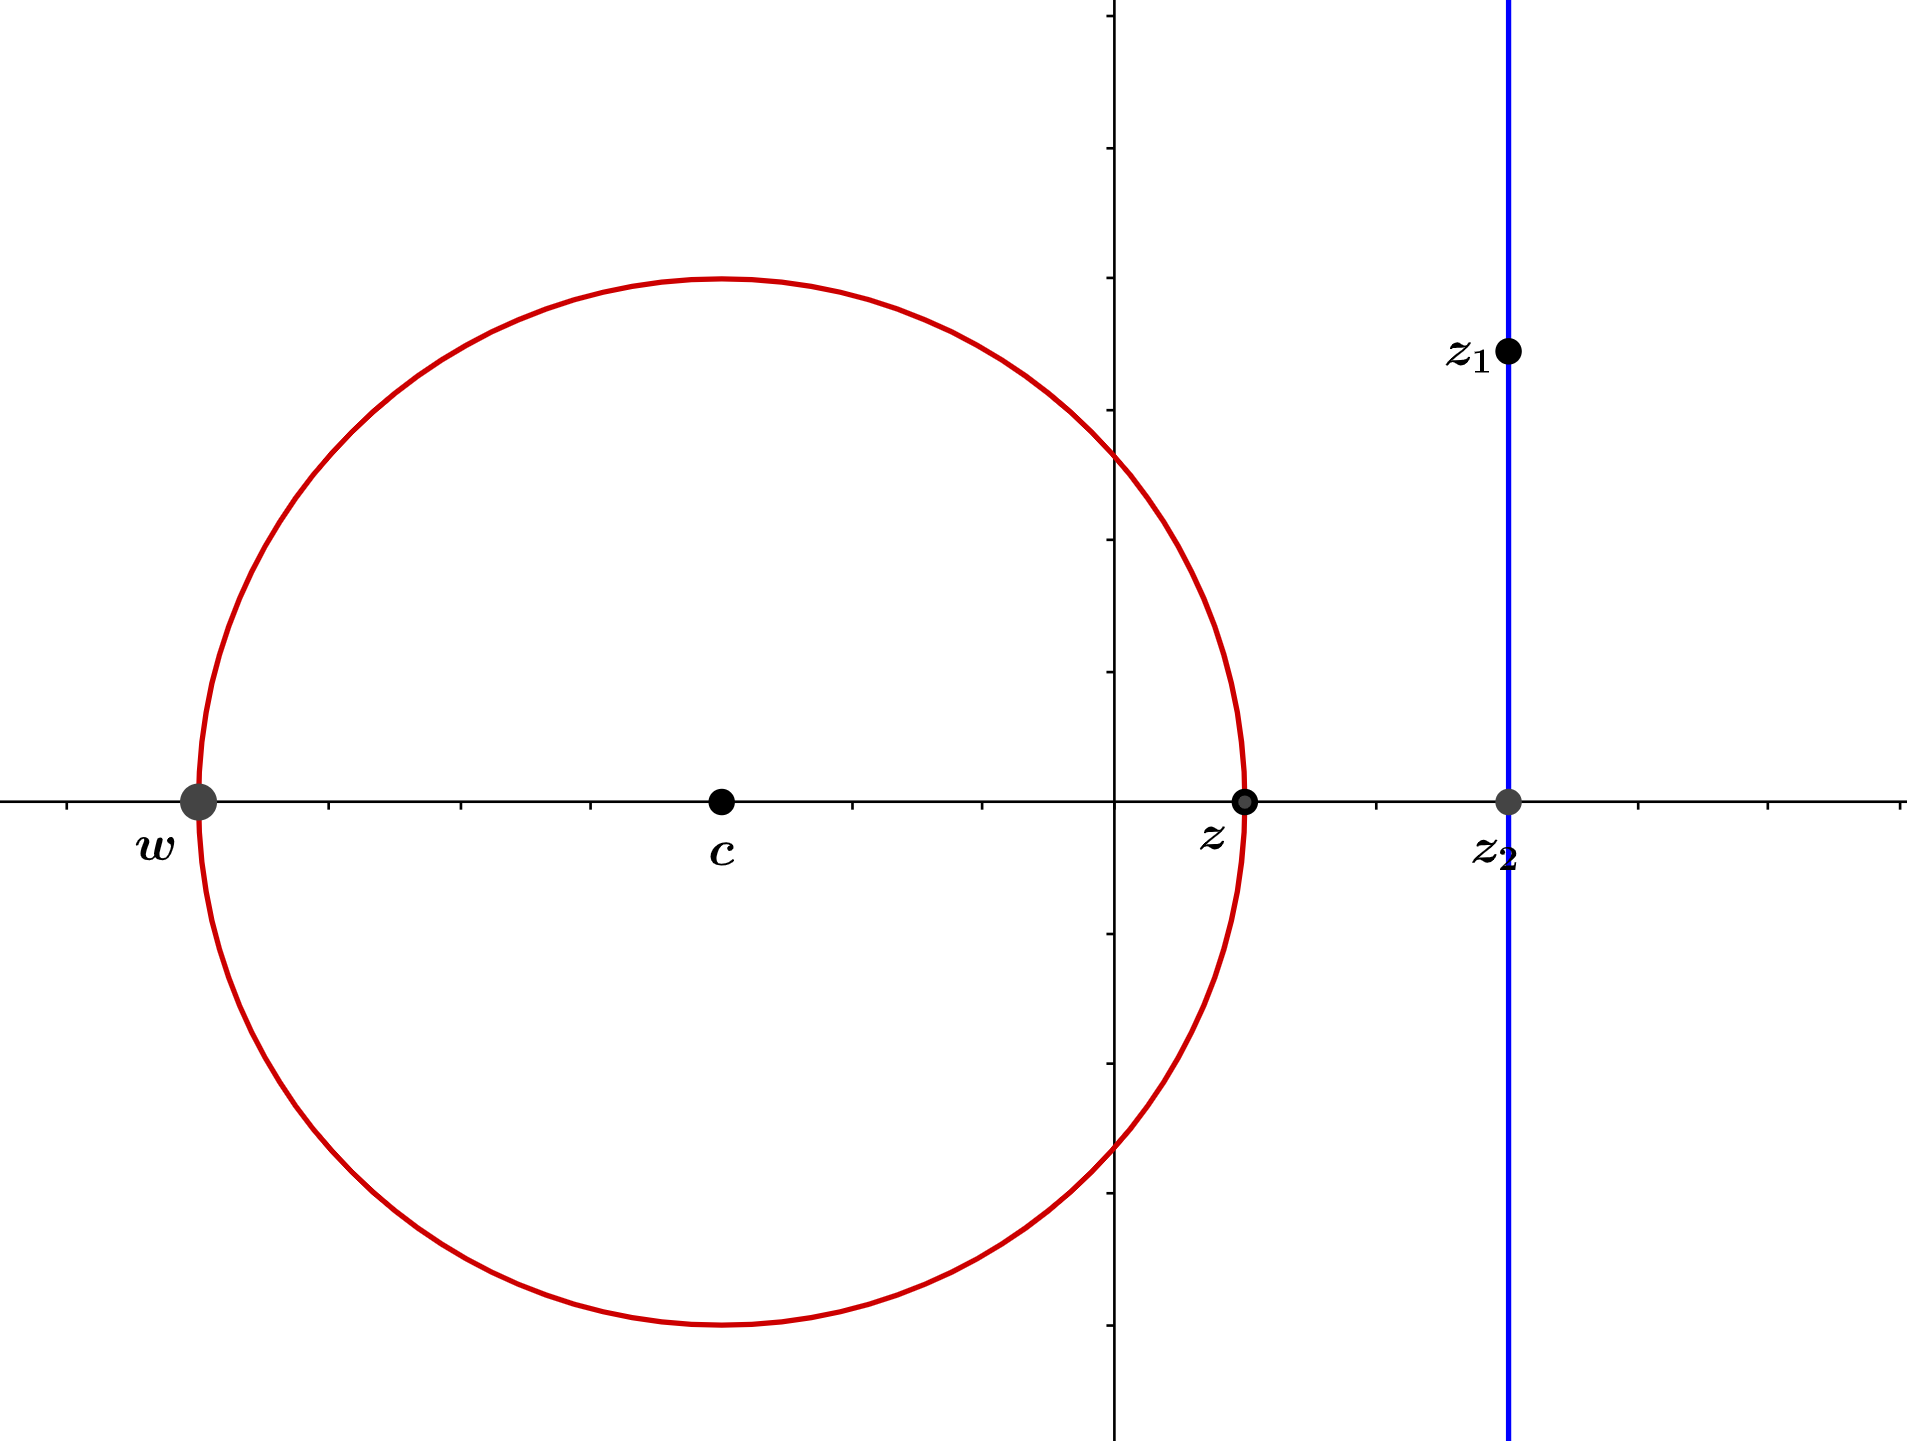
\includegraphics[width=0.55\linewidth]{images/Đường tròn trực giao R.png}
    \caption{Đường tròn suy rộng trực giao với $P^1(\R)$}
    % \label{fig:enter-label}
\end{figure}
\begin{prop}\label{prop 2.2.10}
    Các đường tròn suy rộng trong $P^1(\C)$ mà trực giao với đường tròn suy rộng $P^1(\R)$ là các đường tròn có phương trình
    \[(z\quad w)H\begin{pmatrix}
        \overline{z}\\ \overline{w}
    \end{pmatrix}\]
    trong đó $H \in \Mat(2,\C)$ là một ma trận Hermite hệ số thực.
\end{prop}
\begin{proof}
    Giả sử $C$ là một đường tròn suy rộng trong $P^1(\C)$. Khi đó, theo mệnh đề \ref{prop 2.2.7} thì ma trận Hermite tương ứng của $C$ là 
    \begin{itemize}
        \item $H = \begin{pmatrix}
            1 & -\overline{\alpha}\\
            -\alpha & |\alpha|^2-r^2
        \end{pmatrix}$ nếu $C$ là đường tròn tâm $\alpha$ bán kính $r$.

        Để $C$ trực giao với đường tròn suy rộng $P^1(\R)$ thì tâm $\alpha$ phải thuộc $\R$. Dẫn đến $H$ là một ma trận đối xứng thực. Và do đó là một ma trận Hermite hệ số thực.
        \item $H = \begin{pmatrix}
            0 & e^{-i\theta}\\
            e^{i\theta} & -2r
        \end{pmatrix}$ với $C$ là hợp của một đường thẳng $L$ trong $\C$ với $\{\infty\}$, trong đó $L$ tạo với đường thẳng $\{z\in \C~|~\re(z) = r\}$ góc $\theta$.

        Để $C$ trực giao với đường tròn suy rộng $P^1(\R)$ thì $C$ phải vuông góc với trục thực, tức là $\theta = 0$. Khi đó $H = \begin{pmatrix}
            0 & 1\\
            1 & -2r
        \end{pmatrix}$ là một ma trận đối xứng thực. Và do đó là một ma trận Hermite hệ số thực.
    \end{itemize}
\end{proof}
\begin{cor}\label{prop 2.2.11}
    Cho $A\in \SL(2,\R)$. Phép biến đổi xạ ảnh $T_A: P^1(\C) \to P^1(\C)$ biến một đường tròn suy rộng vuông góc với $P^1(\R)$ thành một đường tròn suy rộng cũng vuông góc với $P^1(\R)$.
\end{cor}
\begin{proof}
    Áp dụng mệnh đề \ref{prop 2.2.8} thì $T_A$ biến một đường tròn suy rộng $C$, có ma trận Hermite tương ứng là $H$, thành một đường tròn suy rộng $C'$, có ma trận Hermite tương ứng là $B^TH\overline{B}$, trong đó $B = A^{-1}$.

    Nếu $C$ trực giao với $P^1(\R)$ thì $H$ là một ma trận Hermite hệ số thực. Mà $B=A^{-1}$ cũng là ma trận hệ số thực nên $\overline{B} = B$. Từ đó $B^TH\overline{B}$ cũng là một ma trận Hermite hệ số thực. Tức là $C'$ cũng trực giao với $P^1(\R)$.

\end{proof}

\begin{defn}
    Một \textbf{đường hyperbolic} của $\hh$ là giao của $\hh$ với một đường tròn suy rộng vuông góc với $P^1(\R)$.
    
    Với $r,s \in P^1(\R)$ là hai điểm phân biệt, kí hiệu $h-line(r,s)$, là đường hyperbolic ứng với đường tròn suy rộng đi qua $r,s$.
\end{defn}
Nhận xét rằng đường hyperbolic $h-line(r_1,s_1)$ trùng với đường hyperbolic $h-line(r_2,s_2)$ khi và chỉ khi $\{r_1,s_1\} = \{r_2,s_2\}$.
\begin{exam*}
    Cho $r,s \in \R$ là hai số thực phân biệt.
    \begin{itemize}
        \item Đường hyperbolic $h-line(r,\infty)$ là một nửa đường thẳng.
        \item Đường hyperbolic $h-line(r,\infty)$ là một trắc địa của $\hh$.
        \item Đường hyperbolic $h-line(r,s)$ là một nửa đường tròn.
    \end{itemize}
\end{exam*}
\begin{lem}\label{lem 2.2.14}
    Tồn tại duy nhất một đường hyperbolic của $\hh$ đi qua hai điểm phân biệt bất kỳ.
\end{lem}
\begin{proof}
    Với $z_1,z_2 \in \hh, z_1 \neq z_2$, khi đó có hai trường hợp xảy ra
    \begin{enumerate}
        \item $\re(z_1) = \re(z_2) = r\in \R$.
        
        Tồn tại duy nhất đường tròn suy rộng $C = \{ z\in \C~|~\re(z) = \re(z_1)\}\cup \{\infty\}$ qua $z_1,z_2$ và vuông góc với $P^1(\R)$. Khi đó $C \cap \hh = h-line(r,\infty)$ là  đường hyperbolic duy nhất qua $z_1,z_2$.
        
        \item $\re(z_1) \neq \re(z_2)$.
        
        Khi đó không tồn tại đường thẳng vuông góc với trục thực qua $z_1,z_2$. Gọi giao điểm duy nhất của trục thực và đường trung trực của đoạn thẳng Euclid nối $z_1,z_2$ là $c$. Khi đó giao của đường tròn suy rộng tâm $c$, bán kính $|c-z_1|$ với $\hh$ chính là nửa đường hyperbolic qua $z_1,z_2$.
        \begin{figure}[htp!]
            \centering
            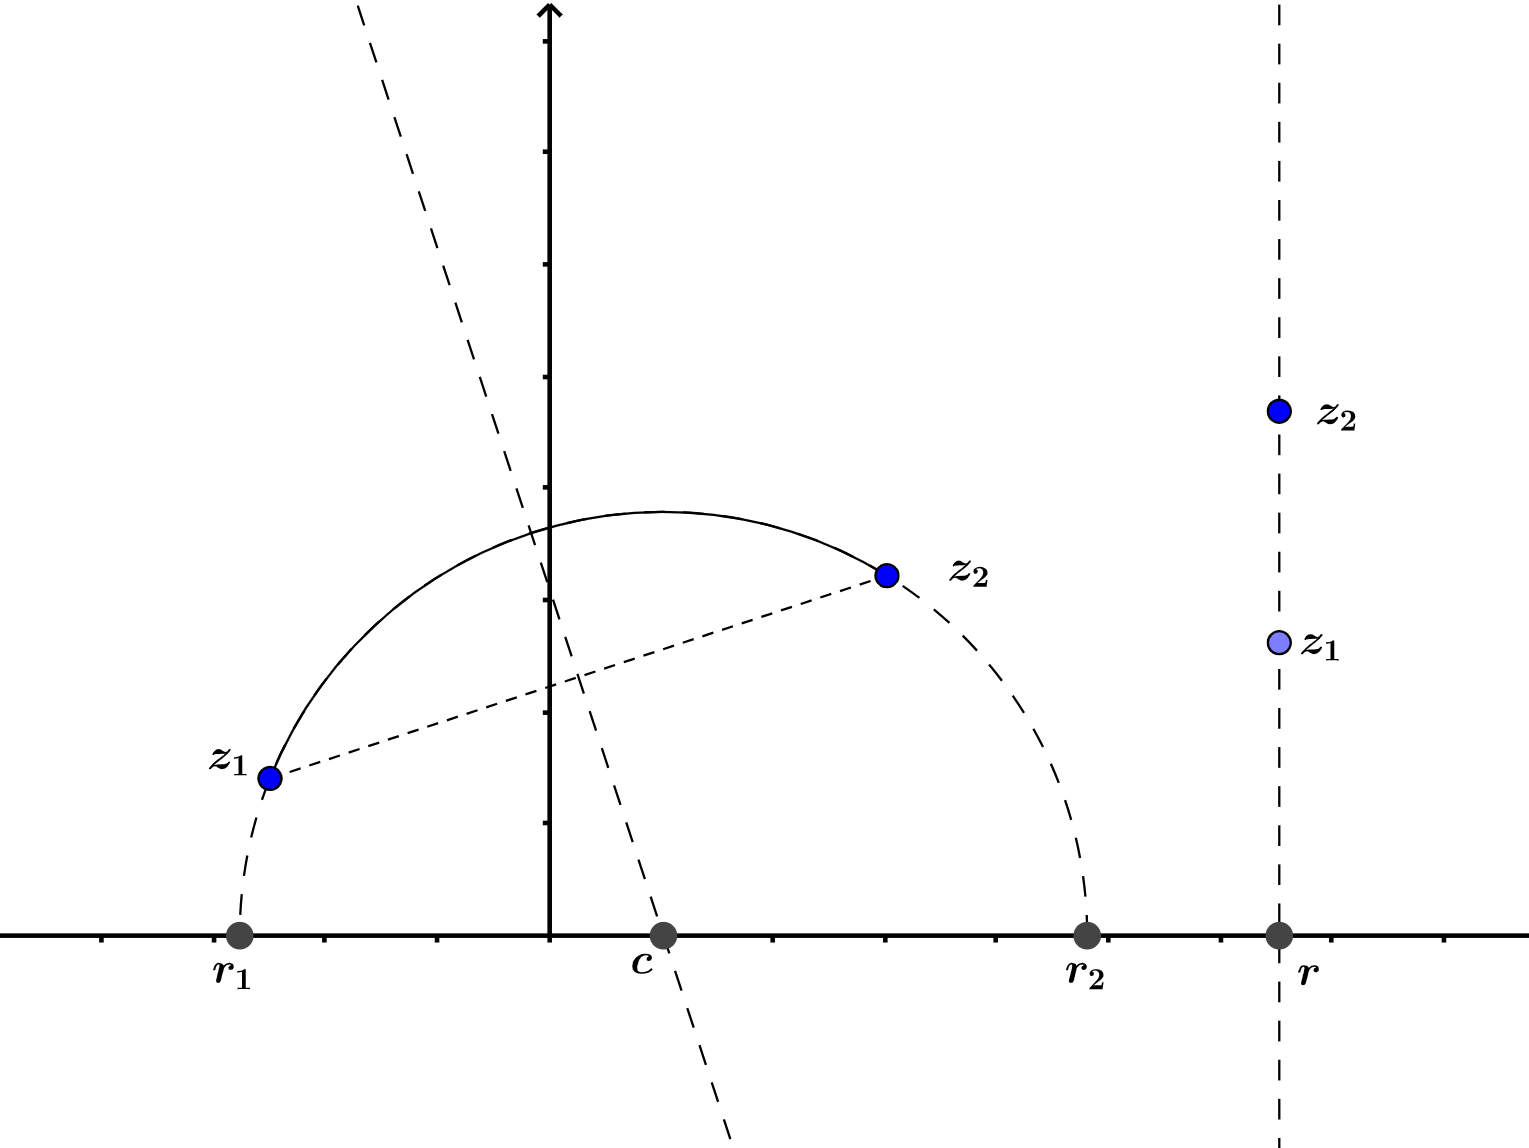
\includegraphics[width=0.5\linewidth]{images/hyperbolic-line.png}
            \caption{Đường hyperbolic trong $\hh$}
            \label{}
        \end{figure}
    \end{enumerate}
\end{proof}
\begin{prop}\label{prop 2.2.15}
    Cho $r,s \in P^1(\R)$. Tồn tại phép biến đổi $T(z) = \dfrac{az+b}{cz+d}$ của $\hh$ biến đường hyperbolic $h-line(r,s)$ thành đường hyperbolic $h-line(0,\infty)$.
\end{prop}
\begin{proof}
    Giả sử $r = [a:b], s = [c:d] \in P^1(\R)$. 
    
    Vì $r \neq s$ nên hai vector $(a,b),(c,d)$ là độc lập tuyến tính trong $\R^2$, do đó $A = \begin{pmatrix}
        a & c\\
        b & d
    \end{pmatrix}$ khả nghịch. 
    
    Đặt $k = \det(A) \neq 0$. Khi đó $\det\begin{pmatrix}
        a/k & b\\
        c/k & d
    \end{pmatrix} = 1$. Dẫn đến $ B = \begin{pmatrix}
        a/k & b\\
        c/k & d
    \end{pmatrix} \in \SL(2,\R)$. Phép biến đổi $T_B(z) = \dfrac{(a/k)z+b}{(c/k)z+d}$ của $\hh$, cảm sinh phép biến đổi xạ ảnh
    \[T_B: P^1(\C) \to P^1(\C),~ [z_1:z_2]\mapsto [(a/k)z_1+bz_2:(c/k)z_1+dz_2]\]
    Khi đó $[1:0] \mapsto [(a/k):(b/k)] = [a:b]$ và $[0:1]\mapsto [c:d]$, tức $T_B$ gửi $0\mapsto s,~\infty \mapsto r$.

    Dẫn đến phép biến đổi $T_B^{-1}$ gửi $s \mapsto 0,~r\mapsto \infty$. Nghĩa là biến $T_B^{-1}$ biến đường tròn suy rộng $C_{r,s}$ qua $r,s$ và vuông góc với $P^1(\R)$, thành đường tròn suy rộng $C_{0,\infty}$ qua $0,\infty$ và vuông góc với $P^1(\R)$. Do đó $T_B^{-1}$ biến $h-line(r,s)$ thành $h-line(0,\infty)$.
\end{proof}
\begin{cor}\label{cor 2.2.16}
    Tất cả các đường hyperbolic của $\hh$ đều là trắc địa của $\hh$.
\end{cor}
\begin{proof}
    Giả sử $r,s$ là hai điểm phân biệt trong $P^1(\R)$. Khi đó, theo mệnh đề \ref{prop 2.2.15}, tồn tại phép biến đổi $T$ của $\hh$ biến đường hyperbolic $h-line(r,s)$ thành đường hyperbolic $h-line(0,\infty)$.

    Ta đã biết $h-line(0,\infty)$ là một trắc địa trên $\hh$.
    
    Khi đó với mỗi đường cong $\gamma$ có vết trên $h-line(r,s)$ ta có
    \[\rho(\gamma(a),\gamma(b)) \leq h(\gamma|_{[a,b]}) = h(T(\gamma)|_{[a,b]}) = \rho(T(\gamma(a)),T(\gamma(b))) = \rho(\gamma(a),\gamma(b)).\]
    Dẫn đến $\rho(\gamma(a),\gamma(b)) =  h(\gamma|_{[a,b]})$, hay $\gamma$ là một trắc địa của $\hh$. 
    
    Do đó $h-line(r,s)$ cũng là một trắc địa của $\hh$.
\end{proof}
\begin{prop}\label{prop 2.2.17}
    Mọi trắc địa cực đại của $\hh$ đều là một đường hyperbolic của $\hh$.
\end{prop}
\begin{proof}
    Với mọi $p\in \hh$ và $v \in T_p\hh$. Khi đó tồn tại duy nhất một đường trắc địa cực đại $\gamma: I \to \hh$ thoả mãn $\gamma(0) = p, \gamma'(0) = v$. 
    
    Mặt khác qua $p$ có duy nhất một đường hyperbolic tiếp xúc với $v$. Thật vậy, nếu $v$ có phương vuông góc với trục thực thì tồn tại duy nhất đường hyperbolic qua $p$ và tiếp xúc với $v$ là $h-line(\re(p),\infty)$. Còn nếu $v$ có phương không vuông góc với trục thực, qua $p$ kẻ đường thẳng vuông góc với $v$, đường thẳng này cắt trục thực tại điểm duy nhất. Giả sử là $c$. Khi đó tồn tại duy nhất một đường hyperbolic qua $p$ và tiếp xúc với $v$ là nửa đường tròn có tâm $c$ và bán kính $|c-p|$.

    Mặt khác mọi đường hyperbolic đều là đường trắc địa trong $\hh$. Do đó đường hyperbolic qua $p$ và tiếp xúc với $v$ tại $p$ nói trên chính là đường trắc địa cực đại.
    \begin{figure}[htp!]
        \centering
        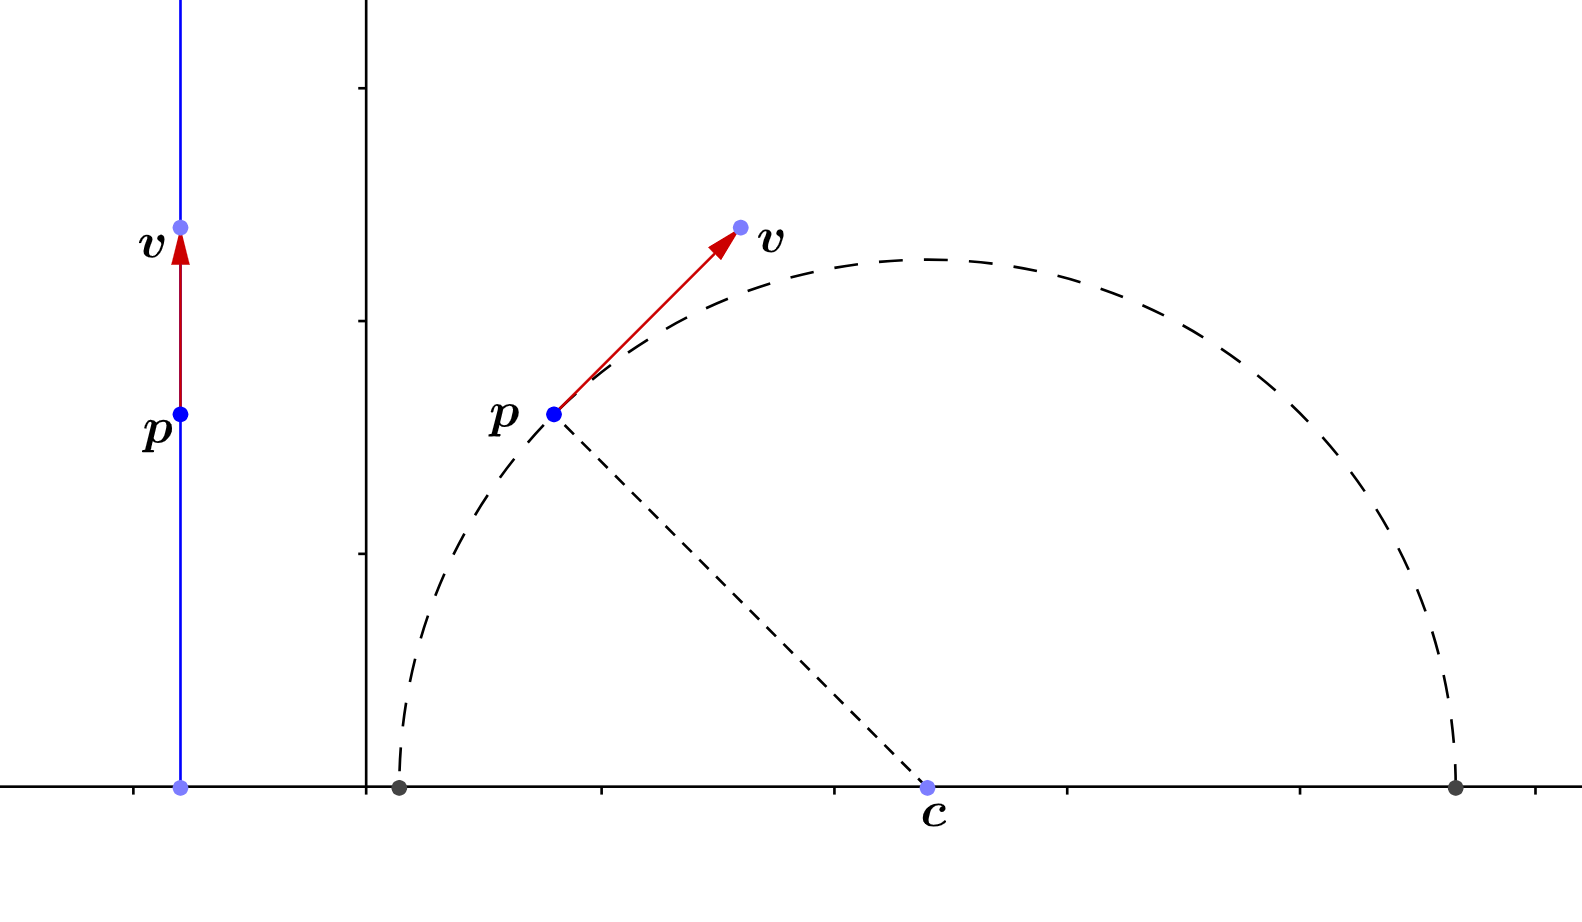
\includegraphics[width=0.5\linewidth]{images/maximum_geodesic.png}
        \caption{đường trắc địa cực đại}
        \label{fig:enter-label}
    \end{figure}
    
\end{proof}
Như vậy, ta đã xác định tất cả các trắc địa cực đại của $\hh$.
\begin{cor}\label{cor 2.2.18}
    Tồn tại duy nhất một trắc địa cực đại của $\hh$ đi qua hai điểm phân biệt bất kỳ.
\end{cor}
\begin{proof}
    Do qua hai điểm bất kì có duy nhất một đường hyperbolic và các đường hyperbolic thì là trắc địa cực đại nên tồn tại duy nhất một trắc địa cực đại của $\hh$ đi qua chúng.
\end{proof}






% \subsection{Đường hyperbolic}
% \begin{defn}[Các đường hyperbolic]

% \begin{enumerate}
%     \item Một \textit{đường thẳng hyperbolic} trong $\hh$ là tập giao của $\hh$ với đường thẳng Euclid vuông góc với trục thực. Nếu giao điểm của đường thẳng trên với trục thực là tại $r\in \R$, thì đường thẳng hyperbolic được kí hiệu bởi $\Axis(r)$. 

%     Nói riêng, $\Axis(0)$ chính là trục ảo của mặt phẳng $\hh$.
    
%     \item Một \textit{nửa đường tròn hyperbolic} trong $\hh$ là tập giao của $\hh$ với một đường tròn Euclid có tâm nằm trên trục thực và cắt trục thực tại 2 điểm phân biệt. Nếu hai giao điểm đó là $r_1,r_2$, thì nửa đường tròn hyperbolic được kí hiểu bởi $\Cir(r_1,r_2)$.
%     \end{enumerate}
% \end{defn}

% \begin{thm}\label{2.2.2}
% Mỗi cặp điểm phân biệt trong $\hh$ có duy nhất một đường hyperbolic đi qua chúng.
% \end{thm}
% \begin{proof}
%     Với $z_1,z_2 \in \hh, z_1 \neq z_2$, khi đó có hai trường hợp xảy ra
%     \begin{enumerate}
%         \item $\re(z_1) = \re(z_2)$.
        
%         Tồn tại duy nhất đường thẳng Euclid $l = \{ z\in \C~|~\im(z) = \re(z_1)\} \subset \C$ qua $z_1,z_2$ và vuông góc với trục thực. Khi đó $\Axis(\re(z_1)) = l \cap \hh $ là  đường thẳng hyperbolic duy nhất qua $z_1,z_2$.
        
%         \item $\re(z_1) \neq \re(z_2)$.
        
%         Khi đó không tồn tại đường thẳng vuông góc với trục thực qua $z_1,z_2$. Gọi giao điểm duy nhất của trục thực và đường trung trực của đoạn thẳng Euclid nối $z_1,z_2$ là $c$. Khi đó giao của đường tròn Euclid tâm $c$, bán kính $|c-z_1|$ với $\hh$ chính là nửa đường tròn hyperbolic qua $z_1,z_2$.
%         \begin{figure}[htp!]
%             \centering
%             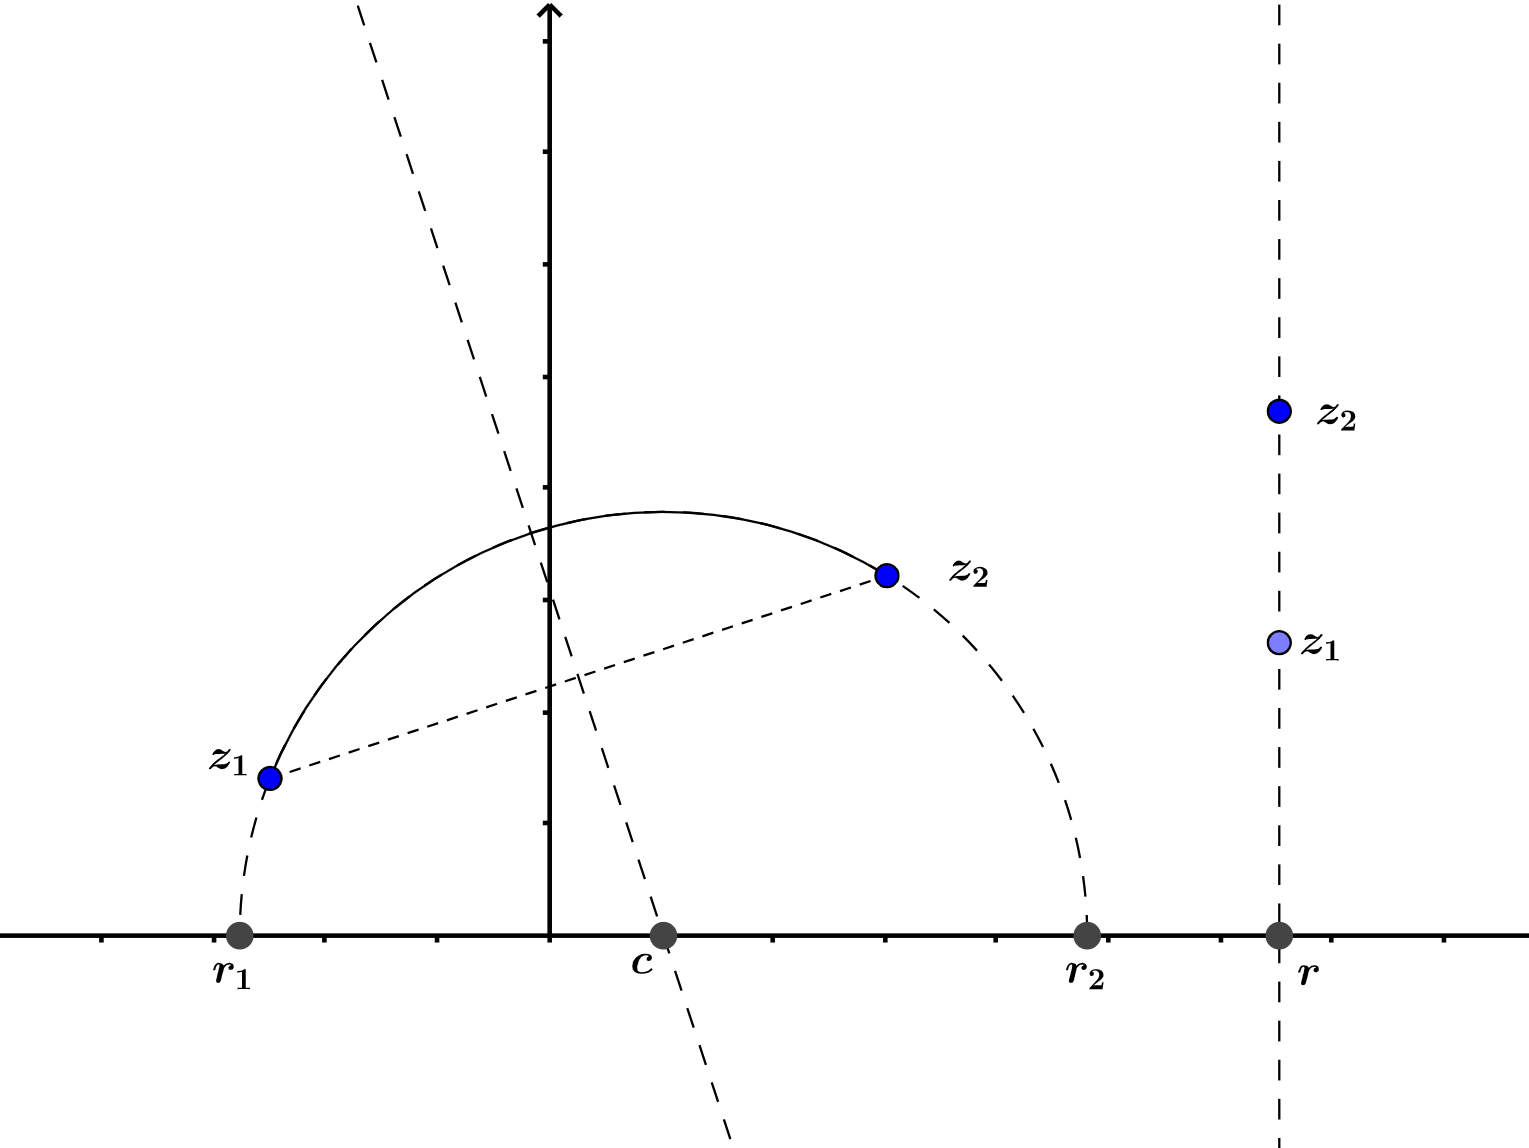
\includegraphics[width=0.6\linewidth]{images/hyperbolic-line.png}
%             \caption{Đường hyperbolic trong $\hh$}
%             \label{}
%         \end{figure}
%     \end{enumerate}
% \end{proof}
% %-------------------------------------------------------------------------
% \begin{thm}\label{thm 2.2.3}
%     Với mọi đường hyperbolic trong $\hh$, tồn tại phép biến đổi trong $\PSL(2,\R)$ biến nó thành trục ảo $\Axis(0)$. 
% \end{thm}
% \begin{proof}
%     \begin{figure}[htp!]
%         \centering
%         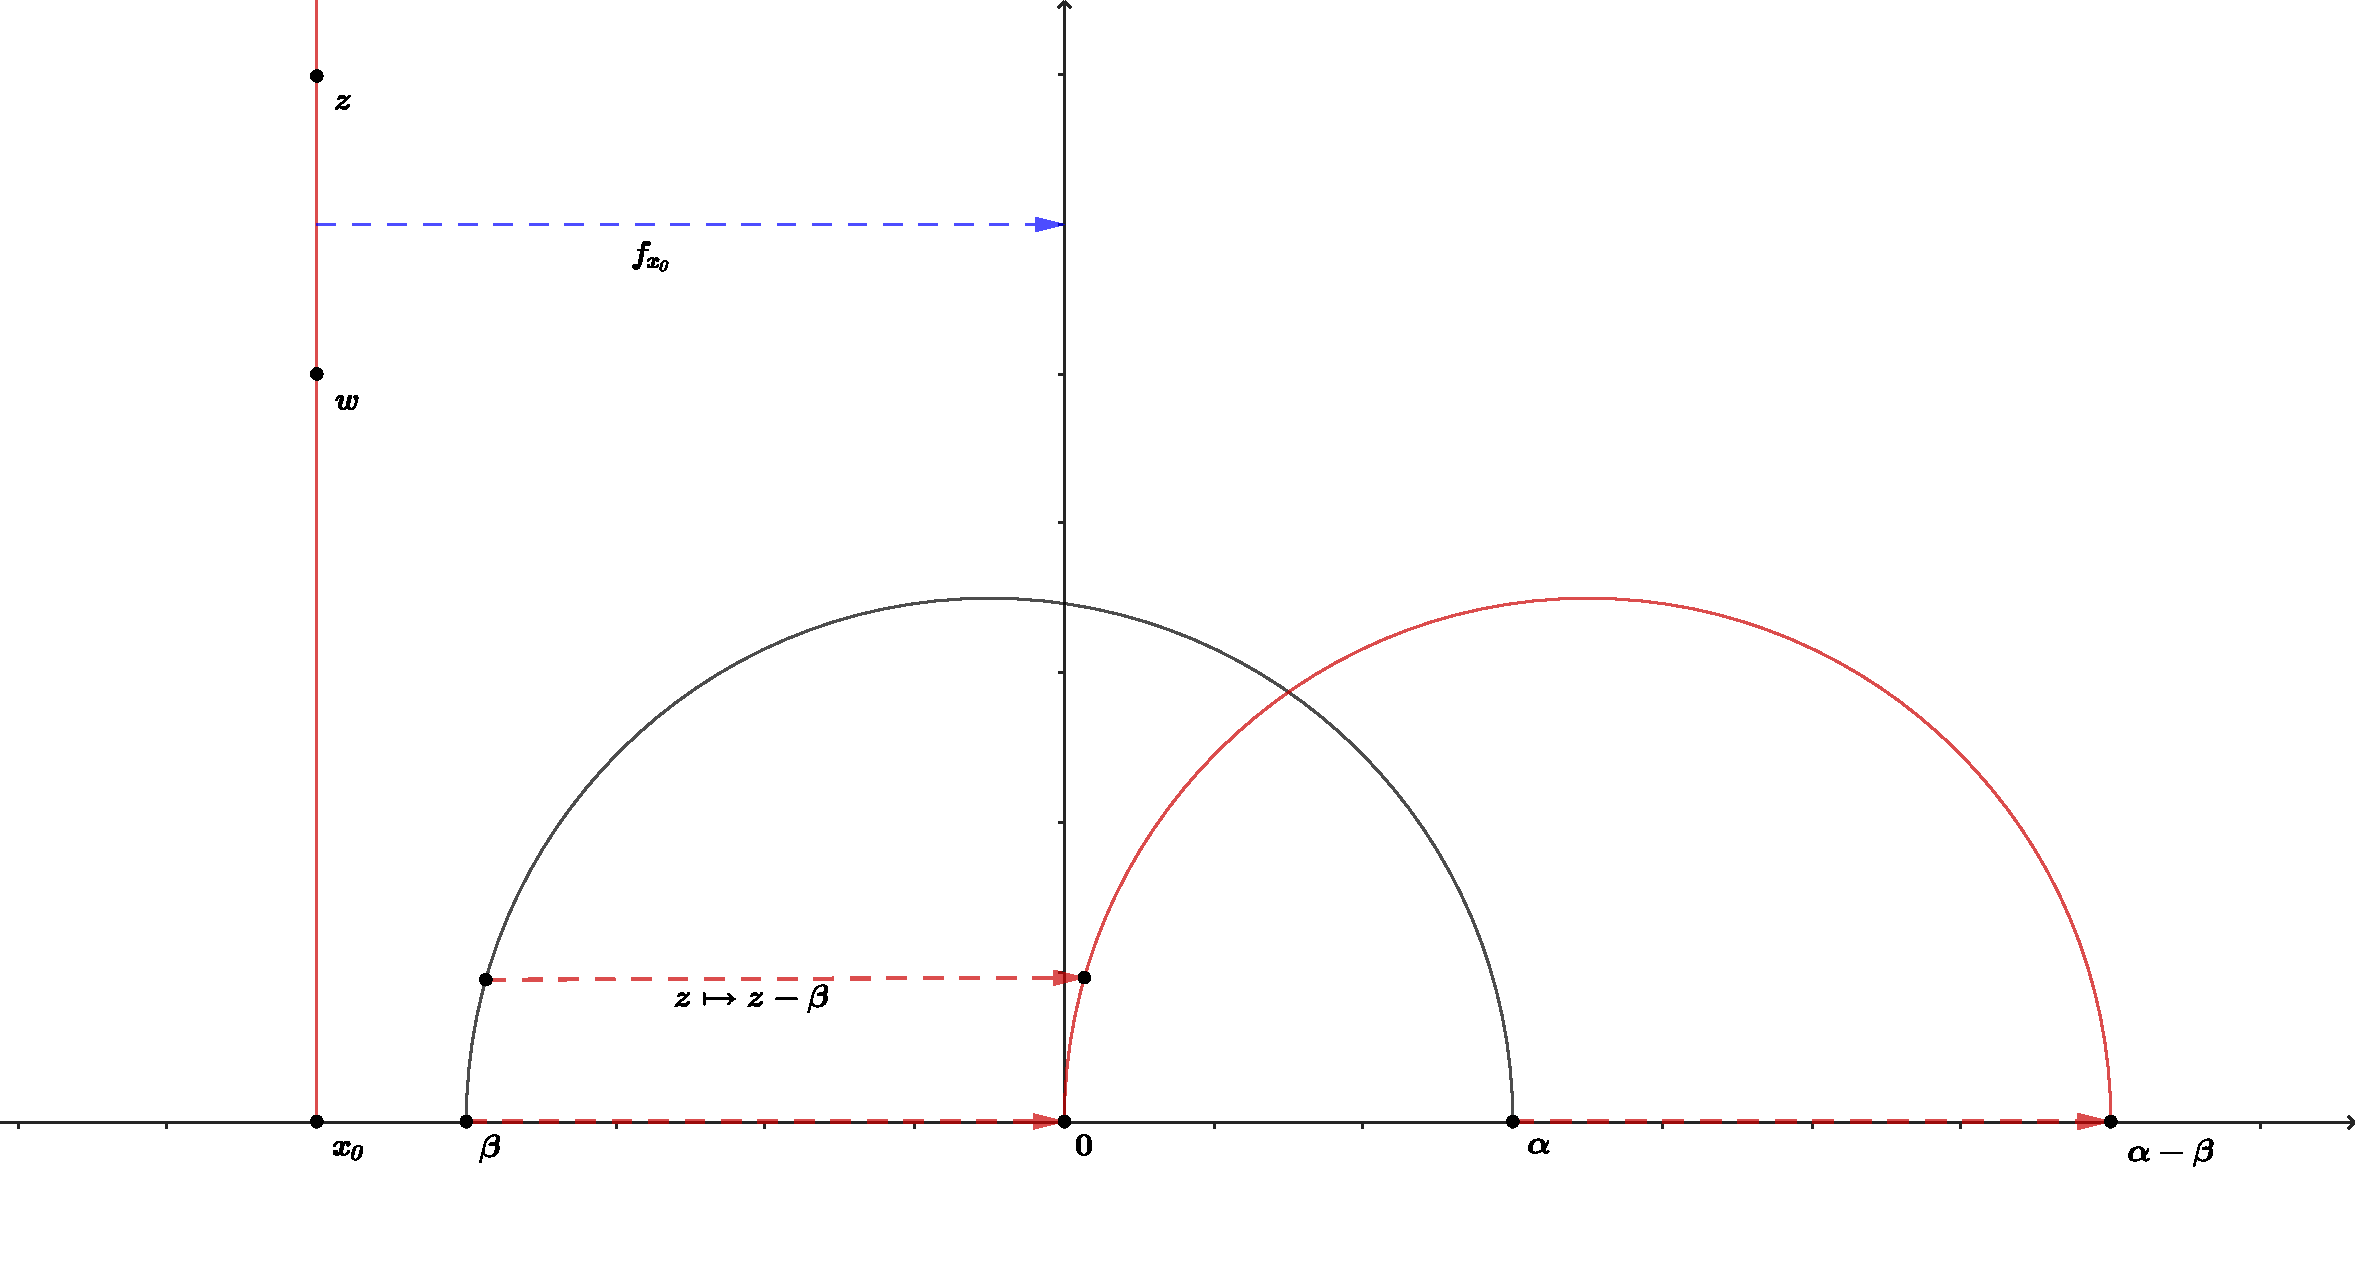
\includegraphics[width=0.75\linewidth]{images/Đường hyperbolic biến thành trục ảo.pdf}
%         \caption{Đường hyperbolic biến thành trục ảo}
%         \label{Đường hyperbolic biến thành trục ảo}
%     \end{figure}
    
%     Xét đường thẳng hyperbolic $\Axis(x_0) = \{x_0 +iy~|~y>0\}\subset \hh$.
    
%     Xét phép biến đổi $T_{x_0}:z \mapsto z-x_0$ trong $\PSL(2,\R)$. Ta có
%     \[T_{x_0}(\Axis(x_0)) = \{T_{x_0}(z)~|~z\in \Axis(x_0)\} = \{(x_0+iy)-x_0 ~|~y>0\}=\{iy ~|~y>0\} = \Axis(0).\]
%     Xét nửa đường tròn hyperbolic $\Cir(\alpha,\beta)$ trong $\hh$.
    
%     Giả sử $\alpha >\beta$, khi đó $\Cir(\alpha,\beta)$ là nửa đường tròn tâm $c = \dfrac{\alpha+\beta}{2}$ và bán kính $r = \dfrac{\alpha - \beta}{2}$. 

%     Với mọi $z\in \Cir(\alpha,\beta)$ thì $\left|z-c\right|= r$, tức là $z = c + re^{i\phi}, \phi \in (0,\pi)$.

%     Xét phép biến đổi $T_{\alpha, \beta}: z\mapsto \dfrac{z-\alpha}{z-\beta}$ trong $\PSL(2,\R)$.
%     Ta có 
%     \begin{align*}
%     T_{\alpha,\beta}(c + re^{i\phi}) &= \dfrac{\dfrac{\alpha - \beta}{2}e^{i\phi}-\dfrac{\alpha - \beta}{2}}{\dfrac{\alpha - \beta}{2}e^{i\phi}+\dfrac{\alpha - \beta}{2}} = \dfrac{e^{i\phi}-1}{e^{i\phi}+1} = \dfrac{(\cos\phi-1)+i\sin\phi}{(\cos\phi+1)+i\sin\phi}\\
%     &= \dfrac{-2\sin^2(\phi/2) + 2i\sin(\phi/2)\cos(\phi/2)}{2\cos^2(\phi/2) + 2i\sin(\phi/2)\cos(\phi/2)}\\
%     &= \dfrac{2i\sin(\phi/2) [\cos(\phi/2)+i\sin(\phi/2)]}{2\cos(\phi/2)[\cos(\phi/2) + i\sin(\phi/2)]}\\
%     & = \tan(\phi/2)i
%     \end{align*}
%     Do đó $T_{\alpha,\beta}(\Cir(\alpha,\beta)) = \left\{\tan(\phi/2)i~|~\phi \in (0,\pi)\right\} =\{it~|~t\in \R_{>0}\} = \Axis(0)$, vì với mỗi $t>0$ có một và chỉ một $\phi \in (0,\pi)$ sao cho $t = \tan(\phi/2).$
% \end{proof}
% \begin{thm}
%     Đoạn trắc địa nối 2 điểm phân biệt $z,w$ trong $\hh$ đều nằm trong đường hyperbolic duy nhất đi qua chúng.
% \end{thm}
% \begin{proof}
%     Xét hai điểm phân biệt $z,w \in \hh$. Khi đó tồn tại duy nhất một đường hyperbolic đi qua $z,w$, gọi là $l_{z,w}$. Theo bổ đề \ref{lem 2.2.4} thì tồn tại một phép biến đổi $T \in \PSL(2,\R)$ biến $l_{z,w}$ thành trục ảo $\Axis(0)$. Giả sử $T(z) = ia, T(w) = ib$ với $0<a<b$.

%     Theo mệnh đề \ref{prop 2.1.8} kết hợp với $T$ là một đẳng cự trong $\hh$ ta được $\rho(z,w) = \rho(T(z),T(w)) = \rho(ia,ib) = \ln{\dfrac{b}{a}}$. Tức đoạn trắc địa giữa $T(z)$ và $T(w)$ chính là
%     là đoạn thẳng Euclid nối $ia, ib$ trên trục ảo chính.

%     Dẫn đến đoạn trắc địa nối $z,w$ phải nằm trên $l_{z,w}$.
    
% \end{proof}
%-------------------------------------------------------------------------
% \begin{lem}
%     Với $z,w \in \hh$ và $f \in \PSL(2,\R)$, ta có
%     \[|f(z)-f(w)| = |z-w|\big|f'(z)f'(w)\big|^{1/2}\]
% \end{lem}
% \begin{proof}
%     Lấy bất kỳ $f\in \PSL(2,\R),~f(z) = \dfrac{az+b}{cz+d}~(ad-bc=1)$, khi đó với mọi $z,w \in \hh$, ta được 
%         \[|f(z) - f(w)| = \dfrac{|z-w|}{|(cz+d)(cw+d)|}.\]
%     Mà $f'(z) = \dfrac{1}{(cz+d)^2}$ và $f'(w) = \dfrac{1}{(cw+d)^2}$ nên
%     $|f(z)-f(w)| = |z-w|\big|f'(z)f'(w)\big|^{1/2}$.
% \end{proof}
%-------------------------------------------------------------------------
Tiếp theo ta có công thức liên quan đến khoảng cách hyperbolic cho 2 điểm bất kỳ trên $\hh$.
\begin{thm}\label{thm 2.2.4}
    Với $z,w \in \hh$, ta có các đẳng thức sau
    \begin{enumerate}
        \item $\rho(z,w) = \ln{\dfrac{|z-\overline{w}|+|z-w|}{|z-\overline{w}|-|z-w|}}$,
        \item $\cosh\rho(z,w) = 1 + \dfrac{|z-w|^2}{2\im(z)\im(w)}$,
        \item $\sinh\left(\dfrac{1}{2}\rho(z,w)\right) = \dfrac{|z-w|}{2(\im(z)\im(w))^{1/2}}$,
        \item $\cosh\left(\dfrac{1}{2}\rho(z,w)\right) = \dfrac{|z-\overline{w}|}{2(\im(z)\im(w))^{1/2}}$,
        \item $\tanh\left(\dfrac{1}{2}\rho(z,w)\right) = \dfrac{|z-w|}{|z-\overline{w}|}\cdot$
    \end{enumerate}
\end{thm}
\begin{proof}
    Lấy bất kỳ $z,w \in \hh$.

    Nếu $z = w$ thì hiển nhiên các đẳng thức cần chứng minh là thoả mãn.
    
    Nếu $z \neq w$, khi đó tồn tại phép biến đổi $f(z) = \dfrac{az+b}{cz+d}$ trong $\PSL(2,\R)$ sao cho 
        \[f(z) = iu,~f(w)=iv~(u>v>0).\]
    Vì $f$ cũng là một đẳng cự nên \[\rho(z,w) = \rho(f(z),f(w)) = \rho(iu,iv) = \ln{\dfrac{u}{v}}\cdot\]
    Do đó
    \[\exp{(\rho(z,w))} =  \dfrac{u}{v},~\exp{(-\rho(z,w))} = \dfrac{v}{u},\]
    \[\exp{\left(\dfrac{1}{2}\rho(z,w)\right)} = \sqrt{\dfrac{u}{v}},~\exp{\left(-\dfrac{1}{2}\rho(z,w)\right)}  = \sqrt{\dfrac{v}{u}}.\]
    Ta lần lượt tính các vế trái của 5 ý trên như sau
    \begin{align*}
         \cosh\rho(z,w) &= \dfrac{\dfrac{u}{v}+\dfrac{v}{u}}{2} = \dfrac{u^2+v^2}{2uv},\\
         \sinh\left(\dfrac{1}{2}\rho(z,w)\right) &= \dfrac{\sqrt{\dfrac{u}{v}}-\sqrt{\dfrac{v}{u}}}{2} = \dfrac{u-v}{2\sqrt{uv}},\\
         \cosh\left(\dfrac{1}{2}\rho(z,w)\right) &= \dfrac{\sqrt{\dfrac{u}{v}}+\sqrt{\dfrac{v}{u}}}{2} = \dfrac{u+v}{2\sqrt{uv}},\\
         \tanh\left(\dfrac{1}{2}\rho(z,w)\right) & = \dfrac{\sinh\left(\dfrac{1}{2}\rho(z,w)\right)}{\cosh\left(\dfrac{1}{2}\rho(z,w)\right)} = \dfrac{u-v}{u+v}.
    \end{align*}
    Tiếp theo ta sẽ tính các vế phải của 5 ý cần chứng minh. 
    
    Ta có $f^{-1}(z) = \dfrac{dz-b}{-cz+a},~\im(f^{-1}(z)) = \dfrac{\im(z)}{|-cz+a|^2}\cdot$
    
    Vì vậy, ta thu được 
    \begin{align*}
        z &= f^{-1}(iu) =\dfrac{-b+i(du)}{a-i(cu)},~\overline{z} =\dfrac{-b-i(du)}{a+i(cu)}\cdot\\
        w &= f^{-1}(iv) =\dfrac{-b+i(dv)}{a-i(cv)},~\overline{w} =\dfrac{-b-i(dv)}{a+i(cv)}\cdot\\
        \im(z) &= \dfrac{u}{a^2+(cu)^2},\quad
        \im(w) = \dfrac{v}{a^2+(cv)^2}\cdot\\
        |z-w|  &= \dfrac{|u-v|}{\sqrt{(a^2+(cu)^2)(a^2+(cv)^2)}},\\
        |z-\overline{w}|  & =\dfrac{|u+v|}{\sqrt{(a^2+(cu)^2)(a^2+(cv)^2)}}\cdot
    \end{align*}
    Ta có các vế phải của 5 ý cần chứng minh lần lượt là 
    \begin{enumerate}
        \item \[\ln{\dfrac{|z-\overline{w}|+|z-w|}{|z-\overline{w}|-|z-w|}}
            = \ln{\dfrac{|u+v|+|u-v|}{|u+v|-|u-v|}}
            = \ln{\dfrac{u}{v}} = \rho(z,w)(\text{do }u>v>0).\]
        % \end{align*}
        \item \[1 + \dfrac{|z-w|^2}{2\im(z)\im(w)} = 1 + \dfrac{|u-v|^2}{2uv} = 1 + \dfrac{(u-v)^2}{2uv} = \dfrac{u^2+v^2}{2uv} = \cosh{\rho(z,w)}.\]
        % \end{align*}
        \item \[\dfrac{|z-w|}{2(\im(z)\im(w))^{1/2}}= \dfrac{u-v}{2\sqrt{uv}} = \sinh\left(\dfrac{1}{2}\rho(z,w)\right).\]
        \item \[\dfrac{|z-\overline{w}|}{2(\im(z)\im(w))^{1/2}}= \dfrac{u+v}{2\sqrt{uv}} = \cosh\left(\dfrac{1}{2}\rho(z,w)\right).\]
        \item \[\dfrac{|z-w|}{|z-\overline{w}|}=\dfrac{u-v}{u+v} = \tanh\left(\dfrac{1}{2}\rho(z,w)\right).\]
    \end{enumerate}
    Từ đó ta có điều phải chứng minh.
\end{proof}
\begin{remark*}
    Từ định lý trên ta thấy, nếu $z_1\neq z_2$ thì $\rho(z_1,z_2) >0$. Điều này kết hợp với những chứng minh ở mệnh đề \ref{prop 2.1.7} nói rằng $\rho$ là một metric trên $\hh$.
\end{remark*}

% \subsection{Đoạn trắc địa}
% \begin{defn}[Đoạn trắc địa]
%     \textbf{Đoạn trắc địa} giữa hai điểm $z,w$ trong $\hh$ là đường cong  có \textit{độ dài hyperbolic ngắn nhất} nối $z$ và $w$, được ký hiệu là $[z,w]$.
    
%     % Khoảng cách của $z,w$ được đo bằng độ dài hyperbolic của đoạn trắc địa đó.
% \end{defn}
% \begin{thm}
%     Đoạn trắc địa nối 2 điểm phân biệt $z,w$ trong $\hh$ đều nằm trong đường hyperbolic duy nhất đi qua chúng.
% \end{thm}
% \begin{proof}
%     Xét hai điểm phân biệt $z,w \in \hh$. Khi đó tồn tại duy nhất một đường hyperbolic đi qua $z,w$, gọi là $l_{z,w}$. Theo bổ đề \ref{lem 2.2.4} thì tồn tại một phép biến đổi $T \in \PSL(2,\R)$ biến $l_{z,w}$ thành trục ảo $\Axis(0)$. Giả sử $T(z) = ia, T(w) = ib$ với $0<a<b$.

%     Theo mệnh đề \ref{prop 2.1.8} kết hợp với $T$ là một đẳng cự trong $\hh$ ta được $\rho(z,w) = \rho(T(z),T(w)) = \rho(ia,ib) = \ln{\dfrac{b}{a}}$. Tức đoạn trắc địa giữa $T(z)$ và $T(w)$ chính là
%     là đoạn thẳng Euclid nối $ia, ib$ trên trục ảo chính.

%     Dẫn đến đoạn trắc địa nối $z,w$ phải nằm trên $l_{z,w}$.
    
% \end{proof}
% %-------------------------------------------------------------------------
% \begin{cor}
%     Khoảng cách hyperbolic giữa $z,w$ bằng độ dài hyperbolic của đoạn trắc địa duy nhất nói trên.
% \end{cor}
%-------------------------------------------------------------------------
\begin{lem}\label{lem 2.2.6}
    Cho $\gamma:[0,1]\to \hh,~\gamma(t) = u(t) + iv(t),~\gamma(0) = ia,~\gamma(1) = c+ib$ là đường cong trơn từng khúc nối $ia,~c+ib ~(c\neq 0<a,b)$ và $\phi:[0,1]\to \hh,~\phi(t) =iv(t)$ là một đường cong trơn từng khúc nối $ia,~ib$. Khi đó $h(\gamma) > h(\phi)$.
\end{lem}
\begin{proof}
    Ta có $\phi(t)=iv(t)$ nên $\im(\phi(t)) = v(t)$ và $|\phi'(t)|=|v'(t)|$. Khi đó
    \begin{align*}
        h(\gamma) = \int_{0}^{1}{\dfrac{\sqrt{(u'(t))^2+(v'(t))^2}}{v(t)}}dt 
        > \int_{0}^{1}{\dfrac{\left|v'(t)\right|}{v(t)}}dt 
        = \int_{0}^{1}{\dfrac{|\phi'(t)|}{\im(\phi(t))}}dt 
        = h(\phi).
    \end{align*}
    % Từ đó suy ra $\rho(ia,ib) < \rho(ia, c+ib)$
\end{proof}
%-------------------------------------------------------------------------
\begin{lem}\label{lem 2.2.7}  
    Cho $z = c+ib,~w=ia \in \hh,~c\neq 0<a,b$. Khi đó $\rho(c+ia, ib) > \rho(ia,ib)$.
\end{lem}
\begin{proof}
     Với $z=c+ib,~w=ia,~c\neq 0<a,b,~b\neq a$ ta được 
    \begin{align*}
        \rho(c+ib,ia) &= \ln{\dfrac{|(c+ib)-(-ia)|+|(c+ib)-(ia)|}{|(c+ib)-(-ia)|-|(c+ib)-(ia)|}}\\
        &= \ln{\dfrac{\sqrt{c^2+(b+a)^2} + \sqrt{c^2+(b-a)^2}}{\sqrt{c^2+(b+a)^2} - \sqrt{c^2+(b-a)^2}}}
    \end{align*}
    \begin{itemize}
        \item Nếu $b=a$ thì \[\rho(c+ib,ia)=\rho(c+ia,ia) = \ln{\dfrac{\sqrt{c^2+(2a)^2} + \sqrt{c^2}}{\sqrt{c^2+(2a)^2} - \sqrt{c^2}}} > \ln{1} = 0 = \rho(ia,ia).\]
        \item Nếu $b\neq a$, do $f(x) = \ln\dfrac{x+1}{x-1},~x>1$ có $f'(x) = \dfrac{-2}{x^2-1} < 0 ~\forall x>1$, nên $f$ là hàm giảm. Do đó với $1<\sqrt{\dfrac{c^2+(b+a)^2}{c^2+(b-a)^2}} < \sqrt{\dfrac{(b+a)^2}{(b-a)^2}}$ thì \[\rho(c+ib,ia)=f\left(\sqrt{\dfrac{c^2+(b+a)^2}{c^2+(b-a)^2}}\right) > f\left(\sqrt{\dfrac{(b+a)^2}{(b-a)^2}}\right) = \rho(ib,ia).\]
    \end{itemize}
\end{proof}
%-------------------------------------------------------------------------
\begin{prop}\label{prop 2.2.8}
    Cho $z,w$ là hai điểm phân biệt trong $\hh$. Khi đó $\rho(z,w) = \rho(z,\xi) + \rho(\xi,w)$ nếu và chỉ nếu $\xi \in [z,w]$.
\end{prop}
\begin{proof}
    Với $z,w \in \hh$ phân biệt, tồn tại phép biến đổi $f \in \PSL(2,\R)$ sao cho \[f(z) = ia,~f(w)= ib~\text{ với } b>a>0 \text{ và } \rho(z,w) =\rho(f(z),f(w)) =\rho(ia,ib)=\ln{\dfrac{b}{a}}\cdot\]
    \begin{figure}[!htp]
        \centering
        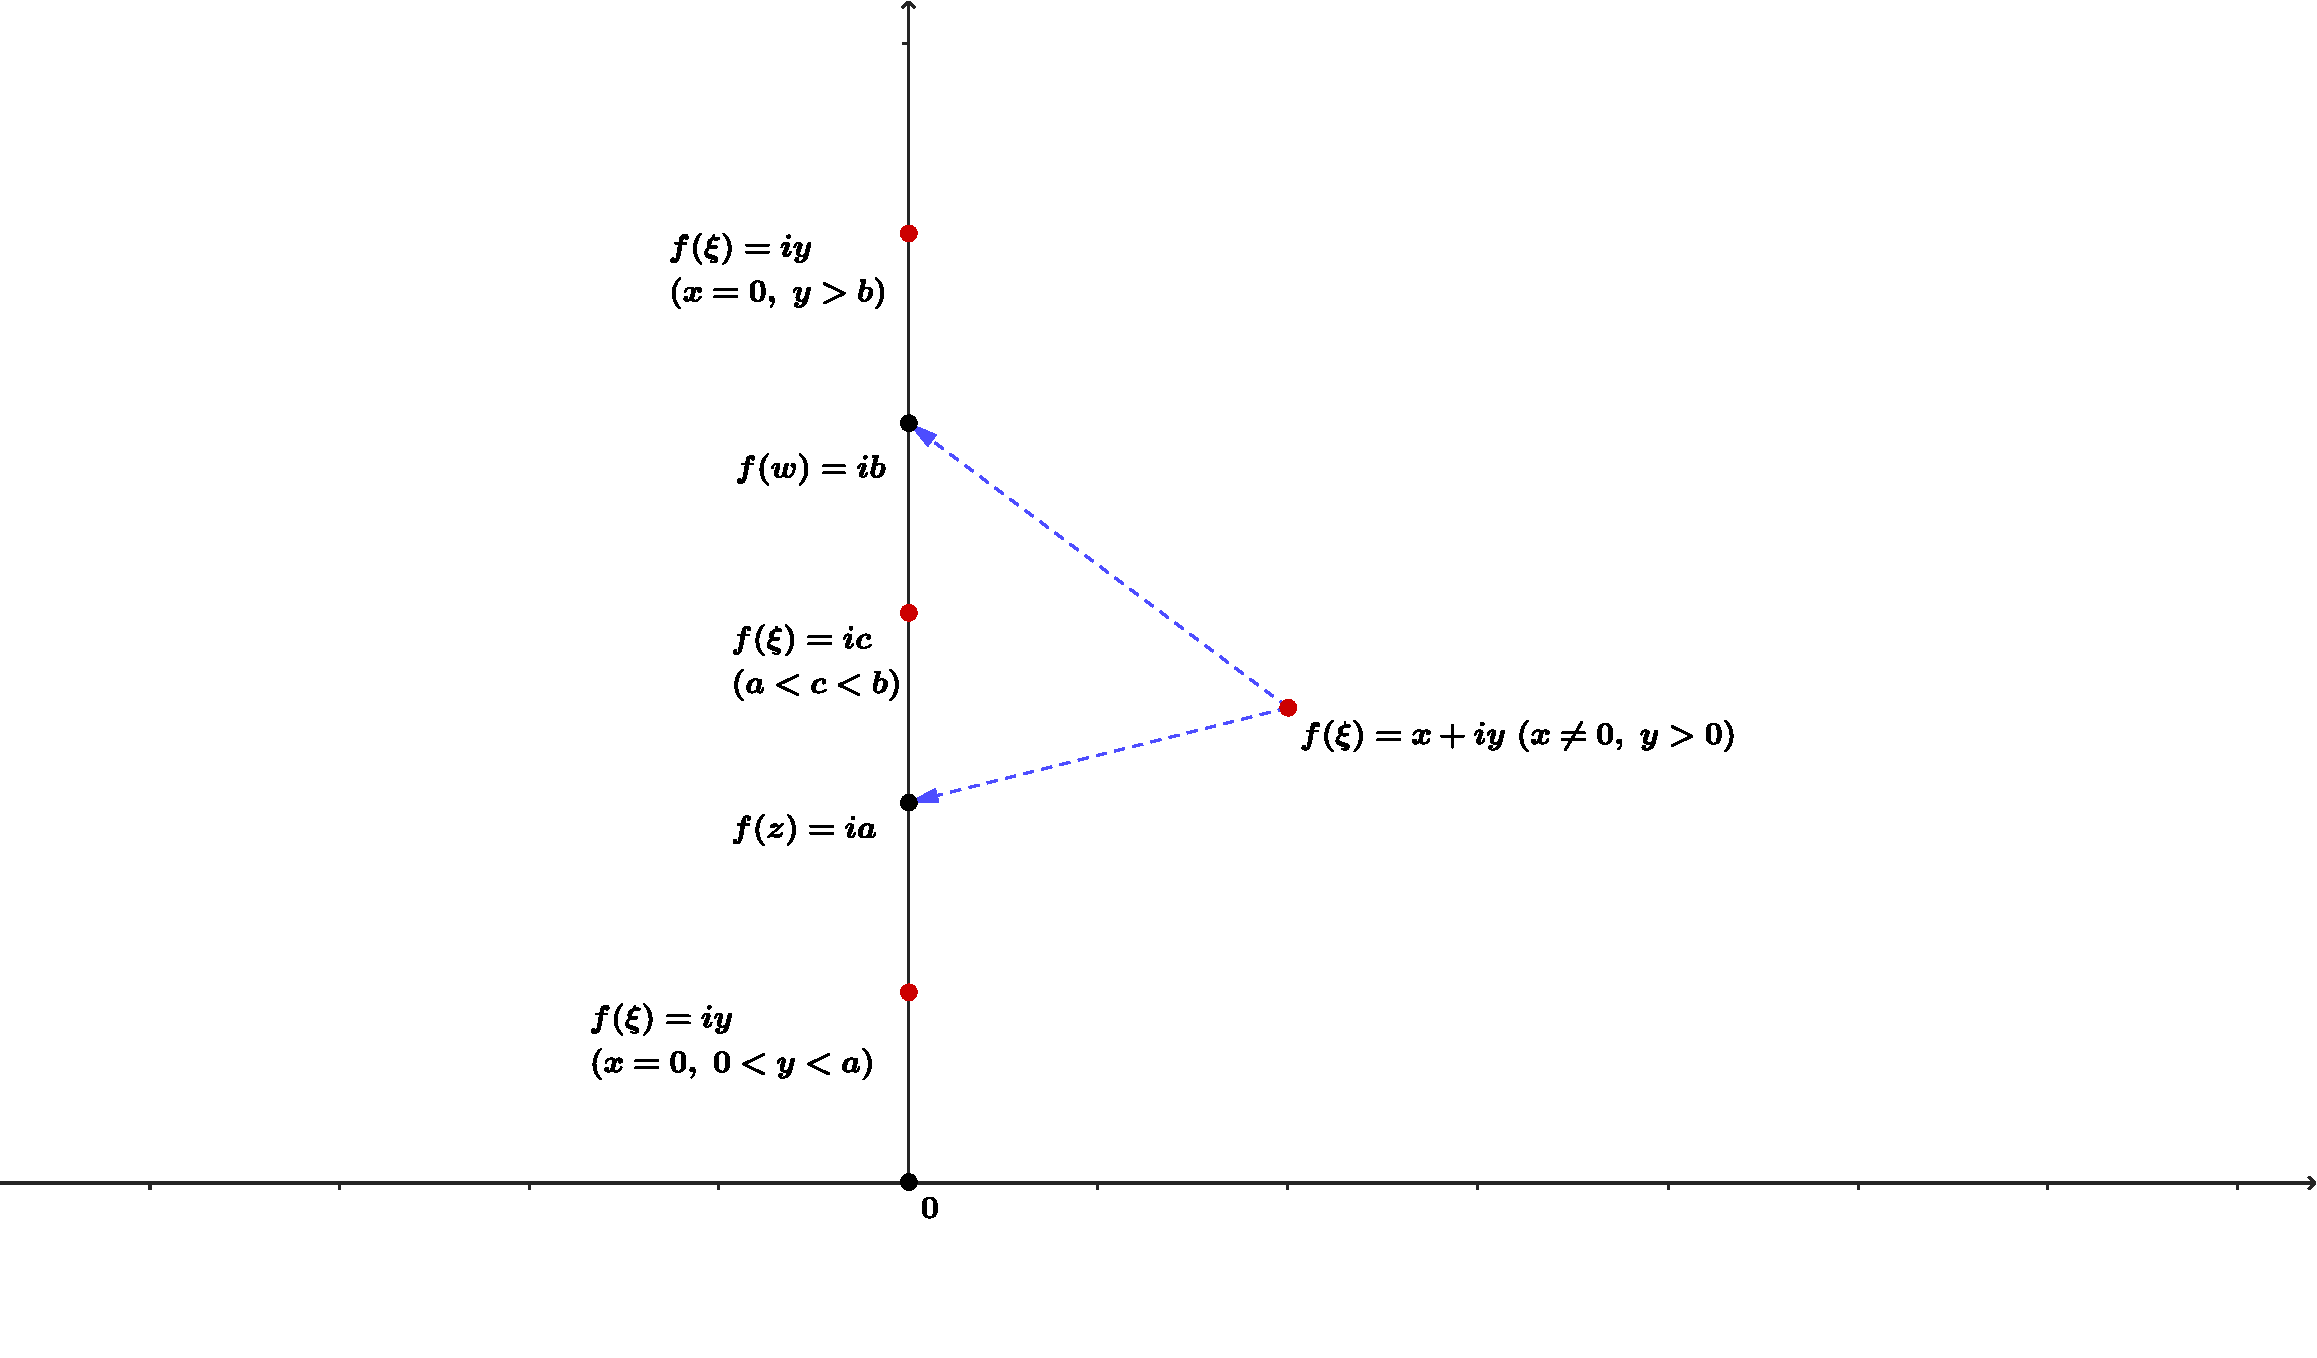
\includegraphics[width=0.6\linewidth]{images/hinh_1.2.1.pdf}
        % \caption{}
        % \label{}
    \end{figure}
    \begin{enumerate}
        \item Nếu $\xi \in [z,w]$ thì $f(\xi) \in [f(z),f(w)]$ nên tồn tại $a<c<b$ sao cho $f(\xi) = ic$. Khi đó 
        \[\rho(z,\xi) = \ln{\dfrac{c}{a}},~\rho(\xi,w) = \ln{\dfrac{b}{c}}\cdot\]
        Suy ra $ \rho(z,\xi) + \rho(\xi,w) = \ln{\dfrac{c}{a}} + \ln{\dfrac{b}{c}} = \ln{\dfrac{b}{a}} = \rho(z,w)$.
        \item Ngược lại, nếu $\rho(z,w) = \rho(z,\xi) + \rho(\xi,w)$, ta cần chứng minh $\xi \in [z,w]$. Giả sử phản chứng $\xi \notin [z,w]$. Đặt $f(\xi) = x+iy~(y>0)$.
        \begin{itemize}
            \item[i)] Nếu $x = 0$ thì $f(\xi) = iy $, do $f$ là song ánh nên $ f(\xi)$ khác $f(z) = ia,~f(w)=ib$, tức $y \neq a,b$, nghĩa là $y > b$ hoặc $0<y<a$. 
            \begin{itemize}
                \item Nếu $y>b$ thì $\rho(z,\xi) + \rho(\xi,w) - \rho(z,w) = \ln{\dfrac{y}{a}} + \ln{\dfrac{y}{b}} - \ln{\dfrac{b}{a}}= \ln{\dfrac{y^2}{b^2}} > \ln{1}=0$.
                \item Nếu $0<y<a$ thì $\rho(z,\xi) + \rho(\xi,w) - \rho(z,w) = \ln{\dfrac{a}{y}} + \ln{\dfrac{b}{y}} - \ln{\dfrac{b}{a}}= \ln{\dfrac{a^2}{y^2}}>\ln{1}=0$.
            \end{itemize}
            Cả hai trường hợp này đều mâu thuẫn với $\rho(z,w) = \rho(z,\xi) + \rho(\xi,w)$.
            \item[ii)] Nếu $x\neq 0$ thì $f(\xi) = x+iy$ không thuộc trục ảo, do đó $f(\xi) \notin [ia,ib]=[f(z),f(w)]$. Khi đó áp dụng bổ đề \ref{lem 2.2.7}
            \begin{itemize}
                \item Nếu $a\leq y \leq b$ thì 
                \begin{align*}
                    \rho(z,\xi) + \rho(\xi,w) - \rho(z,w) &= \rho(ia,x+iy) + \rho(x+iy,ib) - \rho(ia,ib)\\
                    &> \rho(ia,iy) + \rho(iy,ib) -\rho(ia,ib)\\
                    &=\ln{\dfrac{y}{a}} + \ln{\dfrac{b}{y}} - \ln{\dfrac{b}{a}} = 0.
                \end{align*}
                \item Nếu $0<y<a<b$ thì 
                \begin{align*}
                    \rho(z,\xi) + \rho(\xi,w) - \rho(z,w) &= \rho(ia,x+iy) + \rho(x+iy,ib) - \rho(ia,ib)\\
                    &> \rho(ia,iy) + \rho(iy,ib) -\rho(ia,ib)\\
                    &=\ln{\dfrac{a}{y}} + \ln{\dfrac{b}{y}} - \ln{\dfrac{b}{a}} = \ln{\dfrac{a^2}{y^2}} > \ln{1} = 0.
                \end{align*}
                \item Nếu $y>b$
                \begin{align*}
                    \rho(z,\xi) + \rho(\xi,w) - \rho(z,w) &= \rho(ia,x+iy) + \rho(x+iy,ib) - \rho(ia,ib)\\
                    &> \rho(ia,iy) + \rho(iy,ib) -\rho(ia,ib)\\
                    &=\ln{\dfrac{y}{a}} + \ln{\dfrac{y}{b}} - \ln{\dfrac{b}{a}} = \ln{\dfrac{y^2}{b^2}} > \ln{1} = 0.
                \end{align*}
            \end{itemize}
            Cả 3 trường hợp này đều mâu thuẫn với $\rho(z,w) = \rho(z,\xi) + \rho(\xi,w)$.
        \end{itemize}
        Chứng tỏ giả sử phản chứng là sai. Vì vậy $\xi \in [z,w]$.
    \end{enumerate}
\end{proof}
%-------------------------------------------------------------------------
% \begin{prop}\label{prop 2.2.9}
%     Mọi phép biến đổi trong $\PSL(2,\R)$ biến đoạn trắc địa thành đoạn trắc địa trong $\hh$.
% \end{prop}
% \begin{proof}
%     Giả sử $f \in \PSL(2,\R)$ và $z,w$ là hai điểm bất kỳ trong $\hh$ được nối bởi đoạn trắc địa $l = [z,w]$. Khi đó ta cần chỉ ra $f$ tác động lên $l$ thành một đoạn trắc địa trong $\hh$. 
    
%     Thật vậy, với mọi $\xi \in l$ thì 
%     \[\rho(z,w) = \rho(z,\xi) + \rho(\xi,w).\]
%     Mà $f$ là một đẳng cự trong $\hh$ nên
%     \[\rho(f(z),f(w)) =\rho(z,w) = \rho(z,\xi) + \rho(\xi,w)= \rho(f(z),f(\xi)) + \rho(f(\xi),f(w)).\] 
%     Điều này xảy ra khi và chỉ khi $f(\xi) \in [f(z), f(w)]$ là đoạn trắc địa nối $f(z),f(w)$. 
    
%     Chứng tỏ $\forall \xi \in [z,w]$ thì $f(\xi) \in [f(z), f(w)]$, nghĩa là $f$ biến đoạn trắc địa thành đoạn trắc địa trong $\hh$.
% \end{proof}
% \begin{cor}
%     Đoạn trắc địa nối 2 điểm phân biệt $z,w$ trong $\hh$ đều nằm trong đường hyperbolic duy nhất đi qua chúng.
% \end{cor}
% \begin{proof}
%     Xét hai điểm phân biệt $z,w \in \hh$. Khi đó tồn tại duy nhất một đường hyperbolic đi qua $z,w$, gọi là $l_{z,w}$. Tồn tại một phép biến đổi $T \in \PSL(2,\R)$ biến $l_{z,w}$ thành trục ảo $\Axis(0)$. 
    
%     Giả sử $T(z) = ia, T(w) = ib$ với $0<a<b$.
%     Mà đoạn thẳng Euclid nối $ia,ib$ trên trục ảo là đoạn có độ dài hyperbolic nhỏ nhất nối $ia,ib$, cụ thể $\rho(ia,ib) = \ln\dfrac{b}{a}$. 
    
%     Nên đoạn trắc địa $[T(z),T(w)]\subset T(l_{z,w})$ chính là đoạn thẳng Euclid nói trên. Đoạn thẳng này qua ánh xạ nghịch đảo $T^{-1}$ thuộc $l_{z,w}$.
    
%     Mà $T^{-1} \in \PSL(2,\R)$ nên biến đoạn trắc địa thành đoạn trắc địa, 
%     nên $[T^{-1}(ia),T^{-1}(ib)]$ chính là đoạn trắc địa qua $z,w$. 
    
%     Chứng tỏ $[z,w] \in l_{z,w}$.
% \end{proof}
% \begin{remark*}
%     Từ đây, ta thấy mọi đoạn trắc địa đều nằm trên một đường hyperbolic nào đó. Do đó, ta còn gọi đường hyperbolic là đường trắc địa.
% \end{remark*}
% %-------------------------------------------------------------------------
% \begin{cor}
%     Khoảng cách hyperbolic giữa $z,w \in \hh$ bằng độ dài hyperbolic của đoạn trắc địa qua chúng.
% \end{cor}
%-------------------------------------------------------------------------
\subsubsection{Tỉ số kép}
\begin{defn}[Tỉ số kép]
    \textbf{Tỉ số kép} của bốn điểm phân biệt $[z_1:w_1],[z_2:w_2],[z_3:w_3],[z_4:w_4]$ trên đường thẳng xạ ảnh $P^1(\C)$ là 

    \[([z_1:w_1],[z_2:w_2];[z_3:w_3],[z_4:w_4]) = \dfrac{\begin{vmatrix}
         z_1 & z_2\\
         w_1 & w_2
    \end{vmatrix}\begin{vmatrix}
         z_3 & z_4\\
         w_3 & w_4
    \end{vmatrix}}{\begin{vmatrix}
         z_2 & z_3\\
         w_2 & w_3
    \end{vmatrix}\begin{vmatrix}
         z_4 & z_1\\
         w_4 & w_1
    \end{vmatrix}}\in \C\]
\end{defn}
\begin{exam*}
    Tỉ số kép của bốn điểm phân biệt $z_1,z_2,z_3,z_4 \in \C$ là 
    \begin{align*}
        (z_1,z_2;z_3,z_4) &= \dfrac{\begin{vmatrix}
         z_1 & z_2\\
         1 & 1
    \end{vmatrix}\begin{vmatrix}
         z_3 & z_4\\
         1 & 1
    \end{vmatrix}}{\begin{vmatrix}
         z_2 & z_3\\
         1 & 1
    \end{vmatrix}\begin{vmatrix}
         z_4 & z_1\\
         1 & 1
    \end{vmatrix}}
    = \dfrac{(z_1-z_2)(z_3-z_4)}{(z_2-z_3)(z_4-z_1)}\cdot
    \end{align*}
\end{exam*}
\begin{exam*}
    Cho bốn số phức phân biệt $z_1,z_2,z_3,z_4$.
    \begin{enumerate}
        \item Tỉ số kép của bốn điểm $\infty, z_2,z_3,z_4$ là 
        \[(\infty, z_2;z_3,z_4) = ([1:0],[z_2:1];[z_3:1],[z_4:1])=\dfrac{\begin{vmatrix}
         1 & z_2\\
         0 & 1
    \end{vmatrix}\begin{vmatrix}
         z_3 & z_4\\
         1 & 1
    \end{vmatrix}}{\begin{vmatrix}
         z_2 & z_3\\
         1 & 1
    \end{vmatrix}\begin{vmatrix}
         z_4 & 1\\
         1 & 0
    \end{vmatrix}} = \dfrac{(z_3-z_4)}{(z_3-z_2)}.\]

    \item Tỉ số kép của bốn điểm $z_1,\infty,z_3,z_4$ là 
        \[(z_1,\infty;z_3,z_4) = ([z_1:1],[1:0];[z_3:1],[z_4:1])=\dfrac{\begin{vmatrix}
         z_1 & 1\\
         1 & 0
    \end{vmatrix}\begin{vmatrix}
         z_3 & z_4\\
         1 & 1
    \end{vmatrix}}{\begin{vmatrix}
         1 & z_3\\
         0 & 1
    \end{vmatrix}\begin{vmatrix}
         z_4 & z_1\\
         1 & 1
    \end{vmatrix}} = \dfrac{(z_4-z_3)}{(z_4-z_1)}.\]

    \item Tỉ số kép của bốn điểm $z_1,z_2,\infty,z_4$ là 
        \[(z_1,z_2;\infty,z_4) = ([z_1:1],[z_2:1];[1:0],[z_4:1])=\dfrac{\begin{vmatrix}
         z_1 & z_2\\
         1 & 1
    \end{vmatrix}\begin{vmatrix}
         1 & z_4\\
         0 & 1
    \end{vmatrix}}{\begin{vmatrix}
         z_2 & 1\\
         1 & 0
    \end{vmatrix}\begin{vmatrix}
         z_4 & z_1\\
         1 & 1
    \end{vmatrix}} = \dfrac{(z_1-z_2)}{(z_1-z_4)}.\]

    \item Tỉ số kép của bốn điểm $z_1,z_2,z_3,\infty$ là 
        \[(z_1,z_2;z_3,\infty) = ([z_1:1],[z_2:1];[z_3:1],[1:0])=\dfrac{\begin{vmatrix}
         z_1 & z_2\\
         1 & 1
    \end{vmatrix}\begin{vmatrix}
         z_3 & 1\\
         1 & 0
    \end{vmatrix}}{\begin{vmatrix}
         z_2 & z_3\\
         1 & 1
    \end{vmatrix}\begin{vmatrix}
         1 & z_1\\
         0 & 1
    \end{vmatrix}} = \dfrac{(z_2-z_3)}{(z_2-z_1)}.\]
    \end{enumerate}
\end{exam*}

\begin{prop}\label{prop 2.2.15}
    Các phép biến đổi phân tuyến tính của $P^1(\C)$ bảo toàn tỉ số kép. Cụ thể hơn, với bốn điểm phân biệt $P_1,P_2,P_3,P_4$ và phép biến đổi phân tuyến tính $T$ của $P^1(\C)$, ta có
    \[(P_1,P_2;P_3,P_4) = (T(P_1),T(P_2);T(P_3),T(P_4)).\]
\end{prop}
\begin{proof}
    Giả sử $T$ là phép biến đổi phân tuyến tính ứng với ma trận $A\in \GL(2,\C)$. 
    
    Đặt $P_j=[z_j:w_j]$ với $j=1,2,3,4$. Khi đó $T(P_j) = [z'_j:w'_j]$, trong đó $\begin{bmatrix}
        z_j' \\
        w_j'
    \end{bmatrix} = A\begin{bmatrix}
        z_j \\
        w_j
    \end{bmatrix}$.

    Dẫn đến $\begin{bmatrix}
        z_j' & z_k'\\
        w_j' & w_k'
    \end{bmatrix} = A\begin{bmatrix}
        z_j & z_k\\
        w_j & w_k
    \end{bmatrix}$. Do đó $\begin{vmatrix}
        z_j' & z_k'\\
        w_j' & w_k'
    \end{vmatrix} = \det(A)\begin{vmatrix}
        z_j & z_k\\
        w_j & w_k
    \end{vmatrix}$.

    Vì vậy 
    \begin{align*}
        (T(P_1),T(P_2);T(P_3),T(P_4)) &= ([z_1':w_1'],[z_2':w_2'];[z_3':w_3'],[z_4':w_4'])\\
        &= \dfrac{\begin{vmatrix}
         z_1' & z_2'\\
         w_1' & w_2'
    \end{vmatrix}\begin{vmatrix}
         z_3' & z_4'\\
         w_3' & w_4'
    \end{vmatrix}}{\begin{vmatrix}
         z_2' & z_3'\\
         w_2' & w_3'
    \end{vmatrix}\begin{vmatrix}
         z_4' & z_1'\\
         w_4' & w_1'
    \end{vmatrix}}
    = \dfrac{\det(A)\begin{vmatrix}
         z_1 & z_2\\
         w_1 & w_2
    \end{vmatrix}\det(A)\begin{vmatrix}
         z_3 & z_4\\
         w_3 & w_4
    \end{vmatrix}}{\det(A)\begin{vmatrix}
         z_2 & z_3\\
         w_2 & w_3
    \end{vmatrix}\det(A)\begin{vmatrix}
         z_4 & z_1\\
         w_4 & w_1
    \end{vmatrix}}\\
    &= ([z_1:w_1],[z_2:w_2];[z_3:w_3],[z_4:w_4])\\
    &=(P_1,P_2;P_3,P_4).
    \end{align*}
\end{proof}
%-------------------------------------------------------------------------
\begin{thm}\label{thm 2.2.16}
    Cho $z_1\neq z_2$ trong $\hh$. Kí hiệu $z_1^*,z_2^* \in \R \cup \{\infty\}$ là hai giao điểm của đường hyperbolic duy nhất qua $z_1^*,z_2^*$ với $\R \cup \{\infty\}$. Khi đó
    \[\rho(z_1,z_2) = |\ln{(z_2,z_1^*~;~z_1,z_2^*)}|.\]
\end{thm}
\begin{proof}
    Vì $z_1 \neq z_2$ nên tồn tại duy nhất một đường hyperbolic qua $z_1,z_2$ là $h-line(z_1^*,z_2^*)$ với $z_1^*,z_2^*$ là giao điểm với $\R\cup\{\infty\}$. Ta có hai trường hợp sau
    \begin{enumerate}
        \item $z_1^*,z_2^* \in \R,~z_1^*<z_2^*$.

        Xét phép biến đổi $f(z) = \dfrac{z-z_2^*}{z-z_1^*}$ trong $\PSL(2,\R)$ biến $h-line(z_1^*,z_2^*)$ thành $h-line(0,\infty)$. 
        
        Giả sử $f(z_1) = ia, f(z_2) = ib$ với $a,b>0$.
        

        Phép biến đổi này cảm sinh một phép biến đổi xạ ảnh
        \[P^1(\C) \to P^1(\C),\quad [z:w]\mapsto [z-z_2^*w:z-z_1^*w].\]
        Nói riêng 
            $[z_1^*:1]\mapsto [z_1^*-z_2^*:0] = [1:0] \quad
            [z_2^*:1]\mapsto [0:z_2^*-z_1^*] = [0:1]$
        
        Do $f_{z_1,z_2}$ bảo toàn tỉ số kép nên
        \begin{align*}
         (z_2,z_1^*~;~z_1,z_2^*) 
         &= (f([z_2:1]),f([z_1^*:1]);f([z_1:1]),f([z_2^*:1])) \\
         &= ([f(z_2):1],[1,0];[f(z_1):1],[0:1])\\
         % &= ([|f(z_2)|:1],[1,0];[|f(z_1)|:1],[0:1])\\
         &= \dfrac{0-f(z_1)}{0-f(z_2)} = \dfrac{ia}{ib} = \dfrac{a}{b}.
        \end{align*}
        Suy ra $\rho(z_1,z_2) = \rho(f(z_1),f(z_2)) = \rho(ia,ib) = \left|\ln{\dfrac{a}{b}}\right| = |\ln{(z_2,z_1^*~;~z_1,z_2^*)}|$.

        \item Nếu $z_1^* = r \in \R, z_2^* = \infty$. Khi đó $h-line(z_1^*,z_2^*) = h-line(r,\infty)$. Ta có phép biến đổi $T(z) = z-r$ trong $\PSL(2,\R)$ biến $h-line(r,\infty)$ thành $h-line(0,\infty)$. Giả sử $T(z_1) = ia, T(z_2) = ib$ với $a,b>0$.

        Phép biến đổi $T$ cảm sinh một phép biến đổi xạ ảnh trên $P^1(\C)$ là 
        \[P^1(\C) \to P^1(\C),\quad [z:w]\mapsto [z-rw:w].\]
        Nói riêng 
            $[z_1^*:1] = [r:1]\mapsto [0:1], \quad
            [1:0]\mapsto [1:0]$
        
        Do $f_{z_1,z_2}$ bảo toàn tỉ số kép nên
        \begin{align*}
         (z_2,z_1^*~;~z_1,z_2^*) 
         &= (T([z_2:1]),T([z_1^*:1]);T([z_1:1]),T([1:0])) \\
         &= ([T(z_2):1],[0,1];[T(z_1):1],[1:0])\\
         &= \dfrac{0-T(z_1)}{0-T(z_2)} = \dfrac{ia}{ib} = \dfrac{a}{b}.
        \end{align*}
        Suy ra $\rho(z_1,z_2) = \rho(T(z_1),T(z_2)) = \rho(ia,ib) = \left|\ln{\dfrac{a}{b}}\right| = |\ln{(z_2,z_1^*~;~z_1,z_2^*)}|$.
    \end{enumerate}
    
\end{proof}
